\documentclass[]{article}

%Language settings
\usepackage[spanish]{babel}

%Paper size and margins
\usepackage[letterpaper,top=2.54cm,bottom=2.54cm,left=2.54cm,right=2.54cm,marginparwidth=1.75cm]{geometry}

%Other packages
\usepackage{amsmath}
\usepackage{graphicx}
\usepackage[colorlinks=true, allcolors=blue]{hyperref}

\title{3. Generador de PWM}
\author{Flores Tun, Jorge David; López Gómez, Wilberth Eduardo; Sánchez Soberanis, Felipe}

\begin{document}
\maketitle

\section{Introducción}

Existen diversos microcontroladores para señales PWM mediante salidas digitales, sin embargo, para esta práctica se desarrolló un circuito modulador PWM analógico, donde se tendrán
cuatro etapas: 

\begin{itemize}
    \item Rectificación
    \item Generador de rampa
    \item La fuente de corriente directa
    \item Modulación/Potencia
\end{itemize}

De igual manera, se emplearán de puntas de osciloscopio para apreciar las gráficas de cada etapa del circuito y poder analizar la salida del PWM.

\section{Marco teórico}

\subsection{PWM}

La modulación por ancho de pulsos de una señal o fuente de energía es una técnica en la que se modifica el ciclo de trabajo de una señal periódica, estos pulsos varían proporcionalmente
a la amplitud de una señal de entrada.

\begin{figure}[htb]
    \centering
    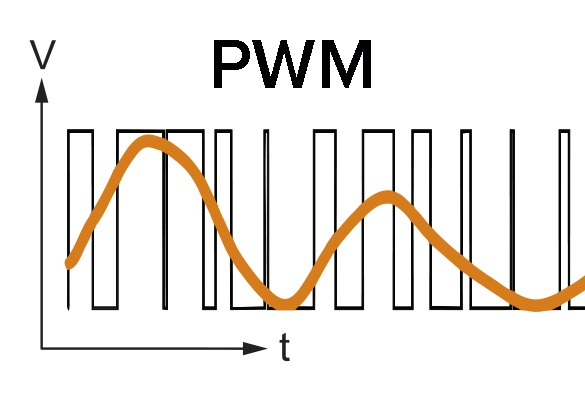
\includegraphics[width=8cm]{build/Imagenes/PWM.jpg}
    \caption{ Gráfica de la modulación por ancho de pulsos}
\end{figure}

\subsection{Puente de Diodos}

Un puente de diodos es una arreglo de cuatro diodos que permiten rectificar una corriente de tipo alterna en corriente continua. El puente visualizado en la figura 2 se le conoce como
rectificador de onda completa o doble onda (Figura 3), ya que rectifica ambos ciclos.

\begin{figure}
    \centering
    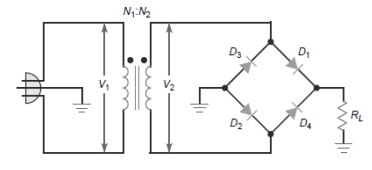
\includegraphics[width=8cm]{build/Imagenes/Rectificador.png}
    \caption{Rectificador de onda completa}
\end{figure}

\begin{figure}
    \centering
    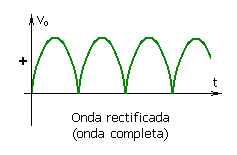
\includegraphics[width=8cm]{build/Imagenes/OndaComp.png}
        \caption{Gráfica de la doble onda}
\end{figure}

\section{Instrucciones}

Elaborar un circuito modulador PWM que permita controlar la potencia entregada a unas carga en la salida del sistema, al igual que obtener las gráficas del sistema requeridas.

\section{Materiales}

\begin{itemize}
    \item Transformador de 12V
    \item Diodo Zener 1N4733
    \item Capacitor electrolítico (10mF)
    \item Capacitor electrolítico (1000$\mu$F)
    \item 5 Diodos 1N4007
    \item Resistencias ($550\Omega y 10K\Omega$)
    \item Potenciómetro (1K$\Omega$)
    \item Transistor NPN
    \item Transistor PNP 
\end{itemize}

\section{Desarrollo}

De manera de crear el circuito visto en clase, se realizó el esquemático en MultiSIM:

\begin{figure}
    \centering
    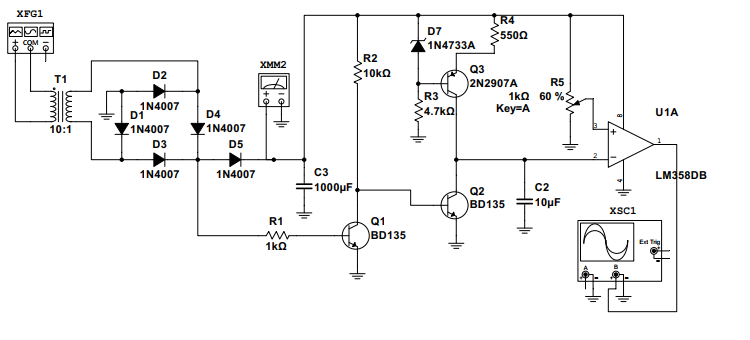
\includegraphics[width=12cm]{build/Imagenes/Circuito.png}
    \caption{Circuito para el PWM}
\end{figure}

Una vez simulado y obteniendo las gráficas deseadas, se realizó el circuito físico, donde se emplearon 2 protoboards para un mayor espacio de trabajo.

\begin{figure}
    \centering
    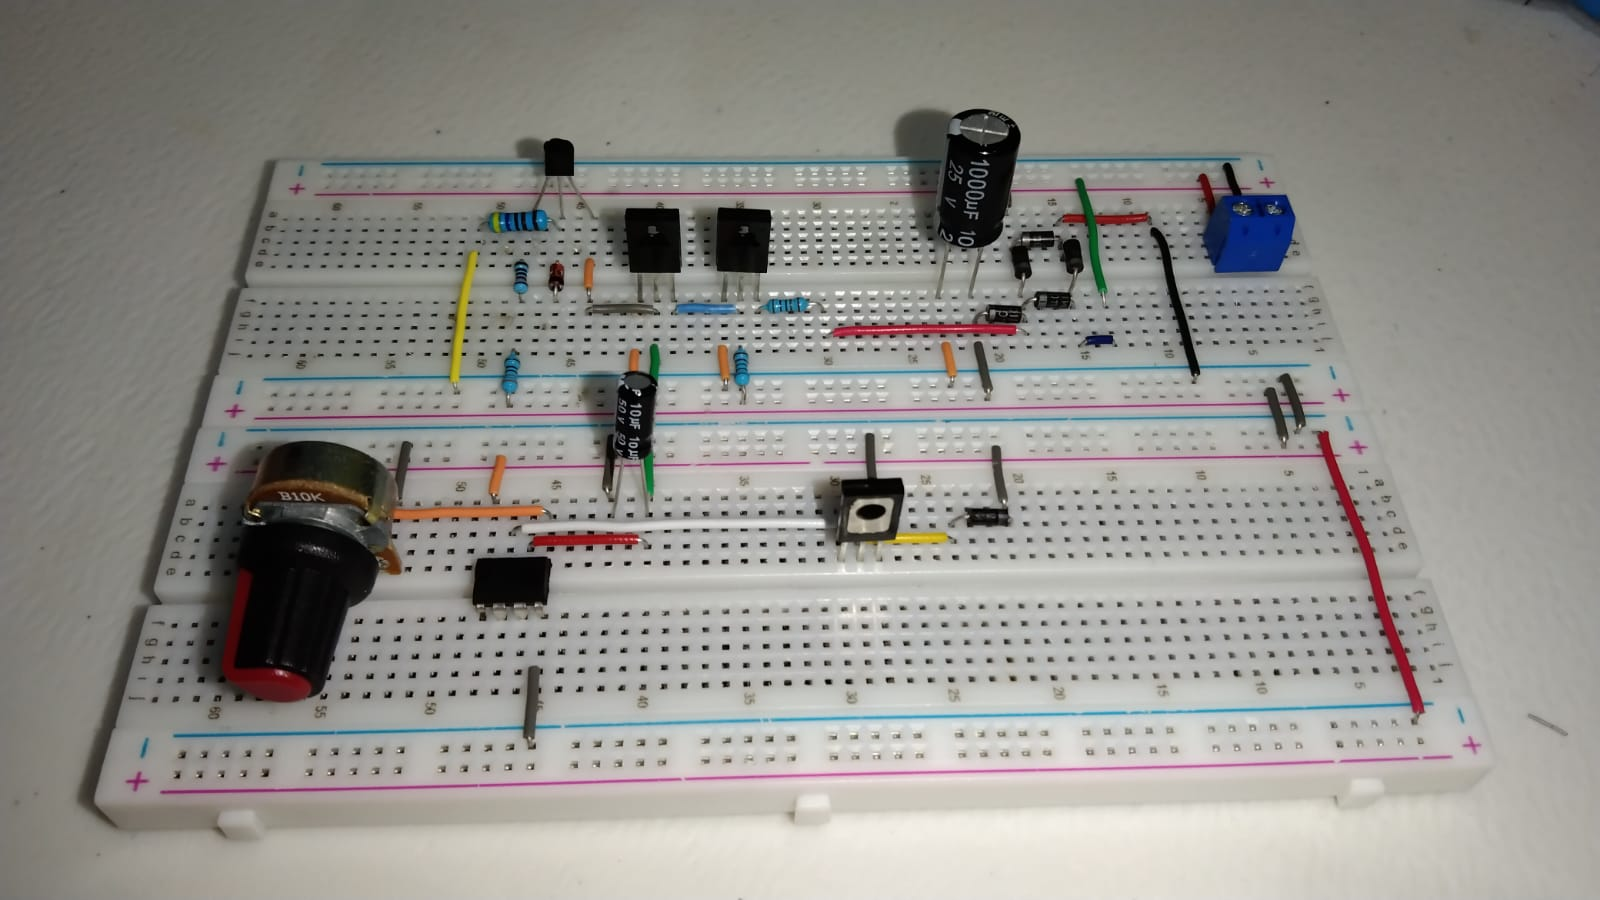
\includegraphics[width=8cm]{build/Imagenes/Circuito3.jpg}
    \caption{Circuito fisico para el PWM}
\end{figure}

Una vez con el circuito armado, se midieron desde distintos nodos del circuito por entradas del osciloscopio para poder visualizar sus gráficas, las cuales son:

\begin{itemize}
    \item Rectificación: En la salida del puente de diodos
    \item DC: Después del diodo individual
    \item PWM: Después del Opamp
    \item Rampa: En la entrada negativa del Opamp
\end{itemize}

\section{Resultados}

Las gráficas obtenidas en el osciloscopio tienen cierta variación al de la simulación, sin embargo, cumplen con los requisitos para aceptar su correcto funcionamiento. 
De igual manera, por medio del potenciómetro, se reguló el ancho de la salida PWM del sistema, el cual podía reflejarse en el osciloscopio.

\begin{figure}
    \centering
    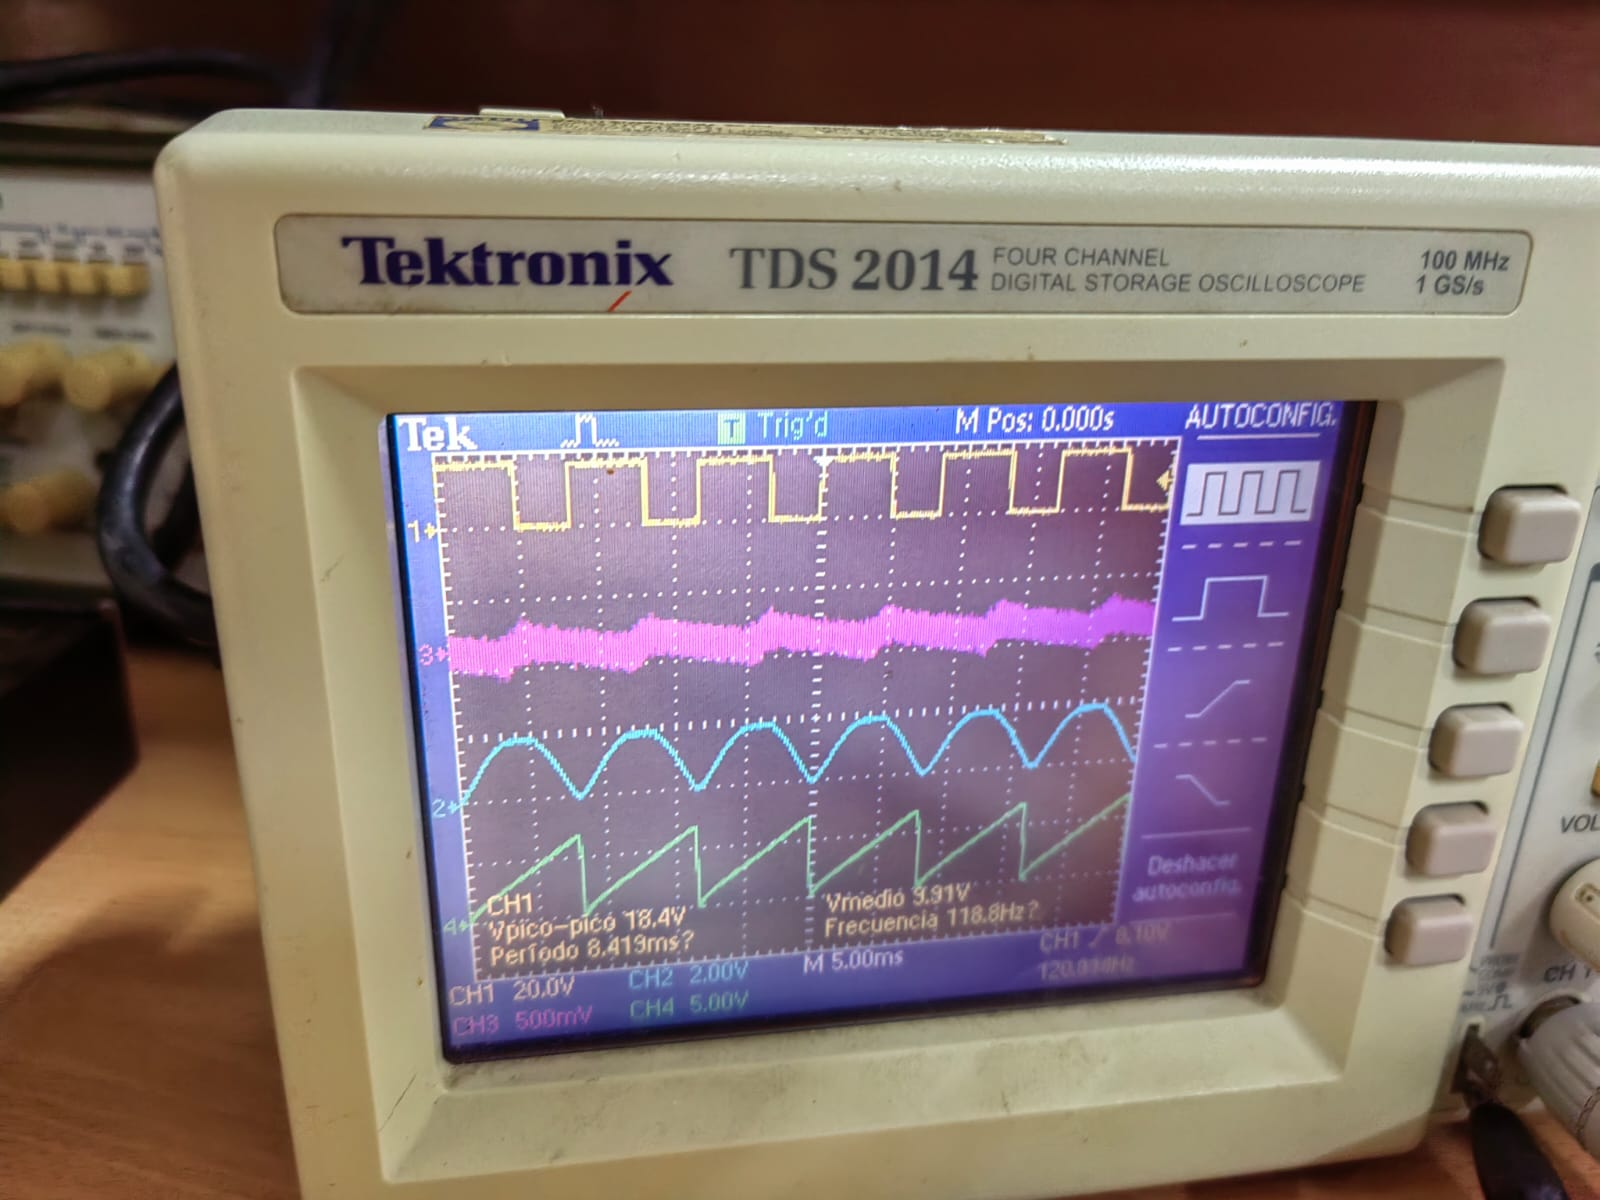
\includegraphics[width=8cm]{build/Imagenes/Resultados.jpg}
    \caption{Gráficas obtenidas en el osciloscopio}
\end{figure}

\section{Conclusiones}

En esta práctica, aprendimos a que podemos generar un PWM a partir de componentes analógicos sin la necesidad de un microcontrolador, esta es una manera eficaz de 
aprender a como desarrollar uno con todas las etapas. De igual manera, la simulación si concordó con los resultados prácticos obtenidos en esta práctica, al igual que las gráficas 
en la simulación en comparación a las prácticas son bastante similares.

\bibliographystyle{alpha}


\end{document}